\chapter{Model Evaluation Methods}\label{sec:usualevaluation}

This chapter introduces several typical model evaluation methods that have been widely applied to various practical applications. Model evaluation is traditionally an integral part of the machine learning model development process. It uses statistical methods to help determine the best machine learning model for a given dataset, and help understand how well the machine learning model will perform in the future. All the evaluations are dependent on the training and test datasets that are collected prior to the model development process. 

\section{Test Accuracy and Error}

Given the input of a machine learning model follows an unknown distribution $P_h$, it is straightforward that we may estimate how good the model is by using a set of data instances sampled from the distribution. 
%
Test accuracy uses a set of test instances $D_{test}$, or test dataset, to evaluate the model $f$ by letting 
\begin{equation}
    Acc(f,D_{test}) = \frac{1}{|D_{test}|}\sum_{(\textbf{x},y)\in D_{test}}(1-\textbf{I}(f(x),y))
\end{equation}
where $\textbf{I}(\cdot,\cdot)$ denotes the 0-1 loss, i.e.,  $\textbf{I}(y_1,y_2)=0$ when $y_1=y_2$, and $\textbf{I}(y_1,y_2)=1$ otherwise. 
%
Moreover, the test error is 
\begin{equation}\label{equ:testerror}
    Err(f,D_{test}) = 1 - Acc(f,D_{test})
\end{equation}

Similar as the above, we can define training accuracy and training error by replacing $D_{test}$ with $D_{train}$. 

\section{Accuracy w.r.t. Training Set Size}

It is interesting to understand, for different machine learning models and different datasets, how the test accuracy changes with respect to the size of the training dataset. Figure~\ref{fig:learning_curve} presents a comparison between decision tree and logistic regression over the California housing dataset. We can see that, in this example, the accuracy of the decision tree increases almost linearly with respect to the size of the training dataset, while the logistic regression increases quickly when the size of the training dataset is small but converges (without a significant increase) afterwards. 

\begin{figure}[!htbp]
    \centering
    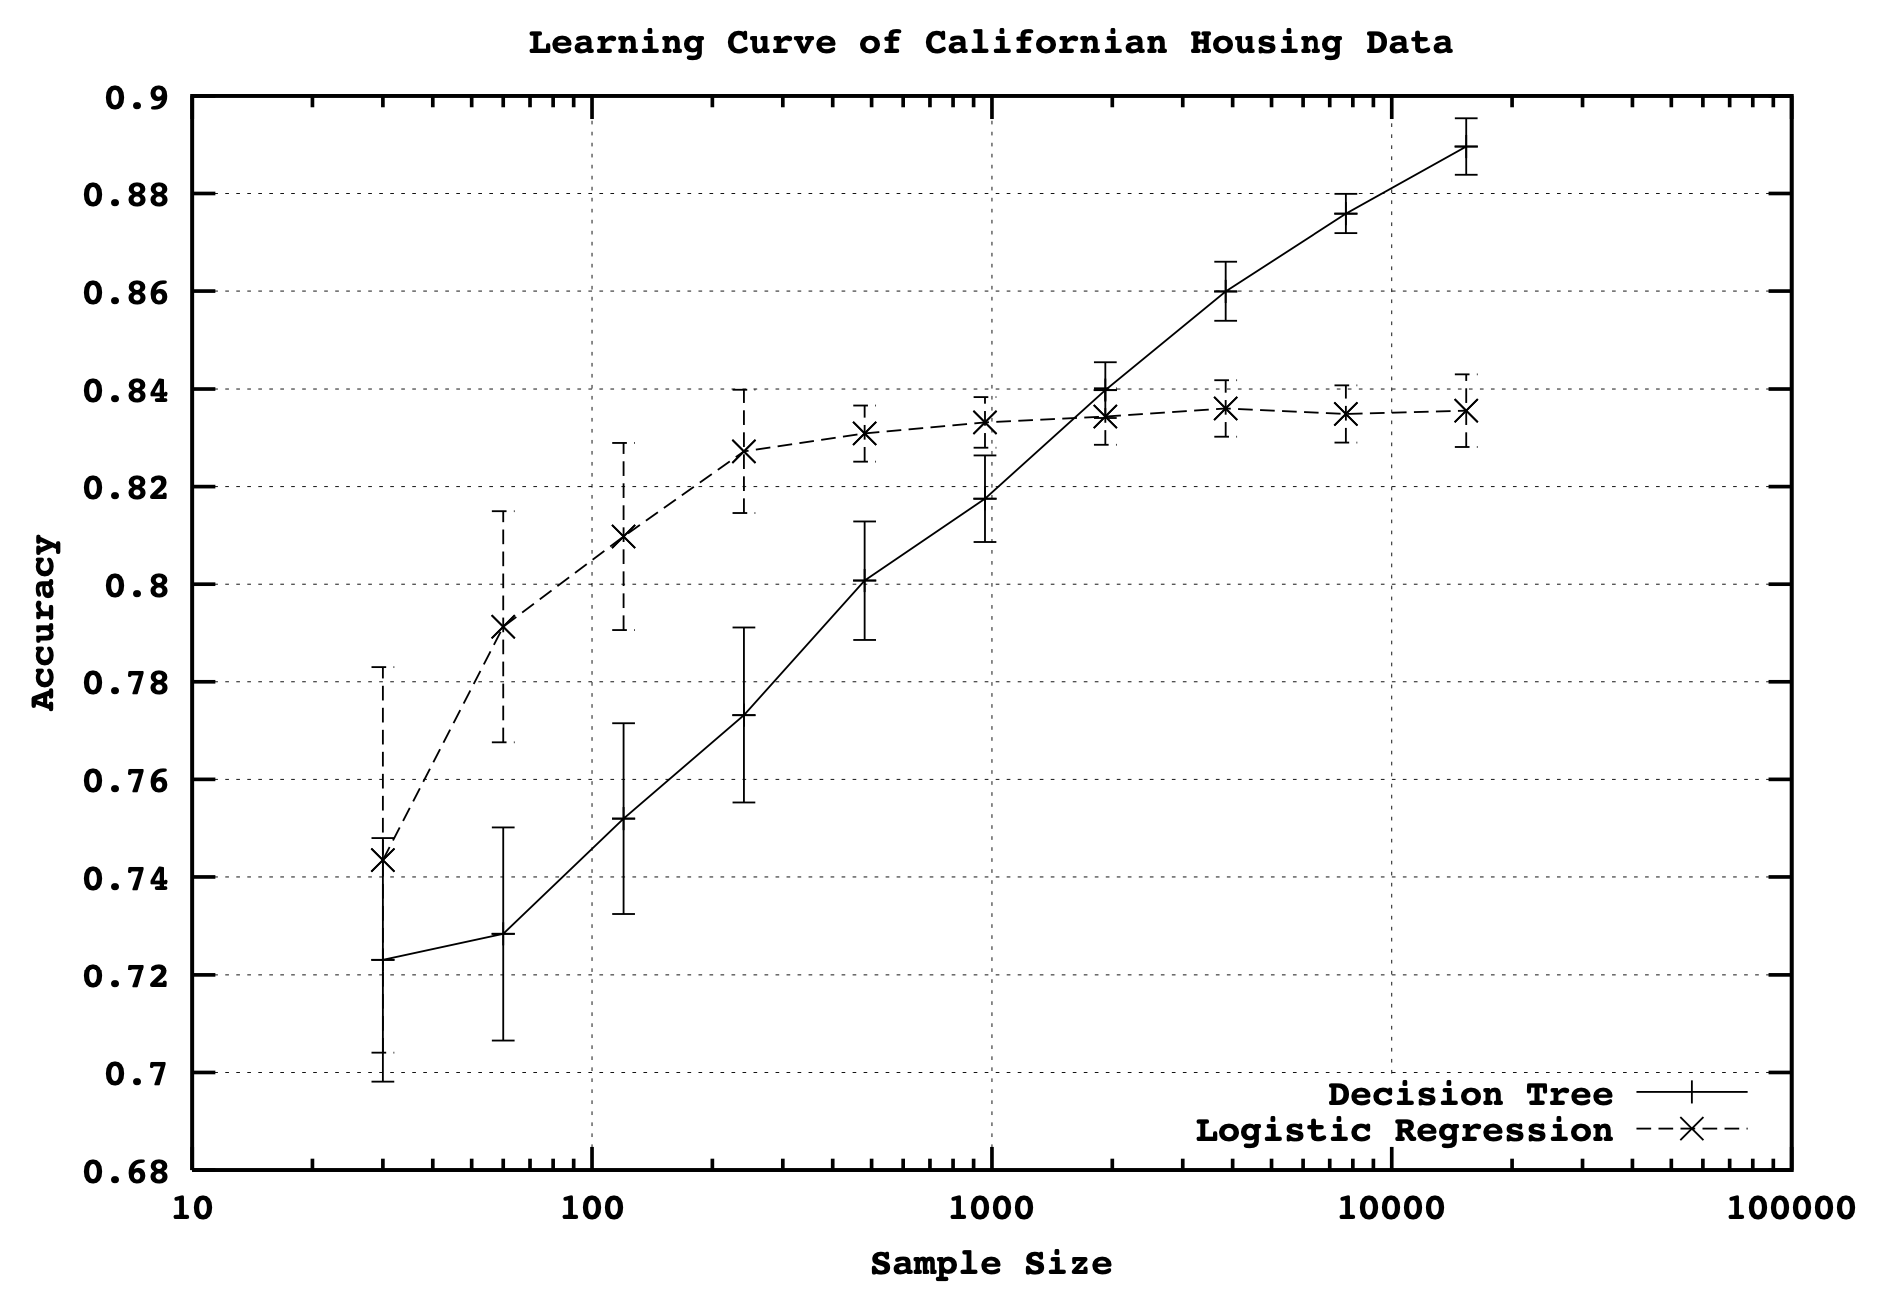
\includegraphics[width=0.7\textwidth]{images/safetyIssues/learningCurve.png}
    \caption{Accuracy w.r.t. Training Set Size \cite{10.1162/153244304322972694}}
    \label{fig:learning_curve}
\end{figure}

\subsection*{How to plot the curve?}

The algorithm proceeds by following Algorithm~\ref{alg:ConstructLearningCurve}. For each sample size $s$, it collects a set of $k$ data into the list $acc$, such that each datum represents a test accuracy of a machine learning model trained over $s$ instances that are randomly sampled from the training dataset. Then, for each number $s$ on the x-axis, we plot a bar of (mean, variance) over the $k$ data. 

\begin{algorithm}
%\KwResult{$S^0_i$ is the spike trains of input $X^0_i$}
\SetAlgoLined

\For{each sample size $s$ on learning curve 
}{
$counter = 0$\\
$acc = []$ \\
\While{$counter < k$}{
randomly select $s$ instances from  $D_{train}$\\
learn a model $f$ \\
evaluate the model $f$ on test set $D_{test}$ to 
               determine accuracy $a$\\ 
$acc$ = $acc.append(a)$\\
$counter = counter + 1$
} 
plot ($s$, average accuracy and 
              error bar) over $acc$
}
 \caption{$\functionname{ConstructLearaningCurve}$($D_{train},D_{test}$), where $D_{train}$ is a set of training instances and $D_{test}$ is a set of test instances}
 \label{alg:ConstructLearningCurve}
\end{algorithm}



\section{Multiple Training/Test Partitions}

For a real-world application, we may not have enough data to make sufficiently large training and test datasets. In this case, the resulting model may be sensitive to the sizes of the datasets. Specifically, a larger test dataset gives us a more reliable estimate of accuracy (i.e., a lower variance estimate), but a larger training dataset will be more representative of how much data we actually have for the learning process. 

In such cases, a single training dataset does not tell us how sensitive accuracy is to a particular training and test split, and we may consider using multiple training/test partitions to evaluate. In the following, we consider several approaches that utilise multiple training/test partitions. 

\subsection*{Random resampling}

We can address the issue by repeatedly randomly partitioning the available data $D$ into training dataset $D_{train}$ and test dataset $D_{test}$. 
%
When randomly selecting training datasets, we may want to ensure that class proportions are maintained in each selected dataset.

\subsection*{Cross validation}

The idea is to partition the data into $k$ subsets, and iteratively leaves one out for test and uses the data in the remaining $k-1$ subsets for training. The resulting accuracy is the average over all the iterations. In general, cross validation makes efficient use of the available data for testing. 
%
In practice, 10-fold cross validation is common, but smaller values of $k$ are often used when learning takes a lot of time.  



\section{Confusion Matrix}\label{sec:confusionmatrix}

Up to now, we have some statistical measurements on roughly how good a model is. However, we have not been able to take a look at what types of mistakes the model makes. To this end, a confusion matrix is often used. The confusion matrix is a matrix where each row represents the number of instances in a \emph{predicted} class, while each column represents the number of instances in an \emph{actual} class (or vice versa). Therefore, those numbers on the main diagonal represent the number of instances whose predictive and true labels are the same, and those numbers not on the main diagonal represent mis-classifications.  


\begin{example}
Equation (\ref{equ:digitsconfusionmatrix}) presents a confusion matrix for the \textbf{digits} dataset over 360 test instances, for a Naive Bayes classifier we trained. We can see that, only four instances are mis-classified, two of them are supposed to be labelled as 1 but classified as 2, one of them is supposed to be 6 but classified as 8, and one of them is supposed to be 9 but classified as 5. 

\begin{equation}
\begin{blockarray}{ccccccccccc}
\begin{block}{c(cccccccccc)}
  \textbf{y=0}~~ & 28 & 0 & 0 & 0 & 0 & 0 & 0 & 0 & 0 & 0 \\
  \textbf{y=1}~~ & 0 & 41 & 0 & 0 & 0 & 0 & 0 & 0 & 0 & 0 \\
  \textbf{y=2}~~ & 0 & 0 & 34 & 0 & 0 & 0 & 0 & 0 & 0 & 0 \\
  \textbf{y=3}~~ & 0 & 0 & 0 & 42 & 0 & 0 & 0 & 0 & 0 & 0 \\
  \textbf{y=4}~~ & 0 & 0 & 0 & 0 & 46 & 0 & 0 & 0 & 0 & 0 \\
  \textbf{y=5}~~ & 0 & 0 & 0 & 0 & 0 & 24 & 0 & 0 & 0 & 1 \\
  \textbf{y=6}~~ & 0 & 0 & 0 & 0 & 0 & 0 & 39 & 0 & 0 & 0 \\
  \textbf{y=7}~~ & 0 & 0 & 0 & 0 & 0 & 0 & 0 & 32 & 0 & 0 \\
  \textbf{y=8}~~ & 0 & 2 & 0 & 0 & 0 & 0 & 1 & 0 & 36 & 0 \\
  \textbf{y=9}~~ & 0 & 0 & 0 & 0 & 0 & 0 & 0 & 0 & 0 & 34 \\
\end{block}
& \textbf{y=0} & \textbf{y=1} & \textbf{y=2} & \textbf{y=3} & \textbf{y=4} & \textbf{y=5} & \textbf{y=6} & \textbf{y=7} & \textbf{y=8} & \textbf{y=9} \\
\end{blockarray}
\label{equ:digitsconfusionmatrix}
\end{equation}
\end{example}

\subsection*{Binary classification problem} 

Consider a binary classification problem. Without loss of generality, we assume that the two classes are $positive$ and $negative$, respectively. Then, we have the following confusion matrix

\begin{equation}
\begin{blockarray}{ccc}
\begin{block}{l(ll)}
  \textbf{y=positive}~~ & \text{true positives (TP)} & \text{false positives (FP)} \\
  \textbf{y=negative}~~ & \text{false negatives (FN)} & \text{true negatives (TN)} \\
\end{block}
& \textbf{y=positive} & \textbf{y=negative} \\
\end{blockarray}
\label{equ:digitsconfusionmatrix}
\end{equation}
where TP denotes the number of true positives, FP the number of false positives, TN the number of true negatives, and FN the number of false negatives. Note that, $|D_{test}| = \text{TP} + \text{FP} + \text{TN} + \text{FP}$

We remark that, in this case, 
\begin{equation}
    Acc(f,D_{test}) =  \frac{\text{TP}+\text{TN}}{|D_{test}|} \text{     and     } Err(f,D_{test}) =  \frac{\text{FP}+\text{FN}}{|D_{test}|}
\end{equation}


\subsection*{Other accuracy metrics} 

Is accuracy an adequate measure of predictive performance? Probably not. For example, when there is a large class negative skew, a high accuracy may be misleading. 

\begin{example}\label{example:truepositive}
For a dataset of 1,000 instances, 97\% of them are supposed to be negative. In this case, a 98\% accuracy may simply be the case that the classifier classifies all negative instances correctly but 2/3 of the positive instances wrongly. This is undesirable for e.g., medical diagnosis, where most of the cases are negative but a true negative may lead to a serious consequence. 
\end{example}



To deal with the problem given in Example~\ref{example:truepositive}, we may consider 

\begin{equation}\label{equ:tp-rate}
    \text{true positive rate (recall)} =  \frac{\text{TP}}{\text{TP}+\text{FN}}
\end{equation}
which focuses on instances whose ground truth are positive. The greater the true positive is, the better the classifier. 

\begin{example}
The recall of the case in Example~\ref{example:truepositive} is 1/98, which means that the classifier does not perform well with respect to recall.
\end{example}

Similarly, we may consider 
\begin{equation}\label{equ:fp-rate}
    \text{false positive rate} =  \frac{\text{FP}}{\text{TN}+\text{FP}}
\end{equation}
which focuses on instances whose ground truth are negative. However, opposite to the case of true positive rate, the smaller the false positive is, the better the classifier. Moreover, we may be interested in  
\begin{equation}\label{equ:positivePrediction}
    \text{positive predictive value (precision)} =  \frac{\text{TP}}{\text{TP}+\text{FP}}
\end{equation}
which focuses on those instances whose predictive values are positive. 

\begin{example}
The false positive rate of the case in Example~\ref{example:truepositive} is 0, and the precision is 1. The classifier performs well in these two metrics. 
\end{example}

\section{Receiver Operating Characteristic (ROC) Curve}

A Receiver Operating Characteristic (ROC) curve plots the true positive rate (Equation~\ref{equ:tp-rate}) vs. the false positive rate (Equation~\ref{equ:fp-rate}) when a threshold on the confidence of an instance being positive is varied. Figure~\ref{fig:ROC-iris} presents an ROC curve on the \textbf{iris} dataset and a logistic classifier. 

\begin{figure}[!htbp]
    \centering
    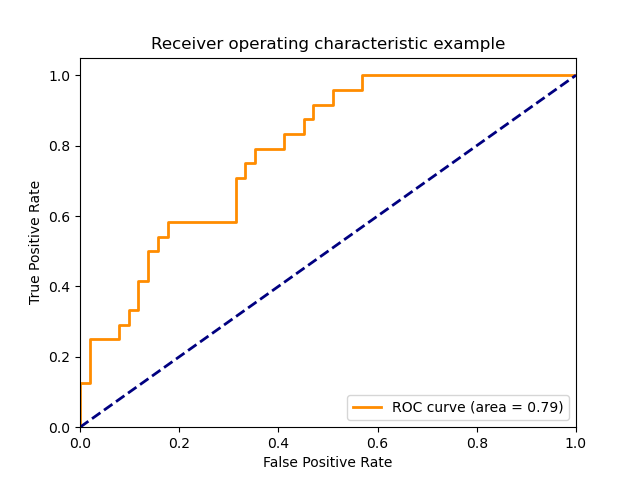
\includegraphics[width=0.6\textwidth]{images/safetyIssues/ROC-iris.png}
    \caption{An ROC curve for \textbf{iris} dataset and a logistic classifier}
    \label{fig:ROC-iris}
\end{figure}

\subsection*{How to plot ROC curve?}

First of all, we can get a function \textbf{calculate\_TP\_FP\_rate(y\_test, y\_test\_preds)} to compute the TP rate and FP rate given the ground truth labels \textbf{y\_test} and the predicted labels \textbf{y\_test\_preds}. Then, the Algorithm~\ref{alg:ROCcurve} enables the computation of a set of (TP rate, FP rate) by working with a set of probability thresholds. The key is to compute predicted labels \textbf{y\_test\_preds} based on the predictions \textbf{y\_predict} and a probability threshold $p$. 

\begin{algorithm}[!htbp]
\SetAlgoLined
probability\_thresholds $= np.linspace(0,1,num=100)$ \\
\For{$p$ in probability\_thresholds}{ 
y\_test\_preds = [] \\
\For{prob in y\_predict}{
\eIf{prob > p}{
y\_test\_preds.append(1)
}{
y\_test\_preds.append(0)
}
}
tp\_rate, fp\_rate = calculate\_TP\_FP\_rate(y\_test, y\_test\_preds)\\
tp\_rates.append(tp\_rate)\\
fp\_rates.append(fp\_rate)
}
\Return tp\_rates, fp\_rates
 \caption{$\functionname{ROC-curve}$(y\_test,y\_predict), where y\_test is the vector of ground truth label, and y\_predict is the vector of predictions}
 \label{alg:ROCcurve}
\end{algorithm}



\subsection*{How to read the ROC curves?}

A skilful model will assign a higher probability to a randomly chosen real positive occurrence than a negative occurrence on average. This is what we mean when we say that the model has skill. Generally, skilful models are represented by curves that bow up to the top left of the plot.
A model with no skill is represented at the point (0.5, 0.5). A model with no skill at each threshold is represented by a diagonal line from the bottom left of the plot to the top right and has an area under curve (AUC) of 0.5.
A model with perfect skill is represented at a point (0,1). A model with perfect skill is represented by a line that travels from the bottom left of the plot to the top left and then across the top to the top right. In general, a greater AUC suggests a better model. 

\section{Precision/Recall (PR) Curves}

A precision/recall curve plots the precision (Equation~\ref{equ:positivePrediction}) vs. recall (Equation~\ref{equ:tp-rate}) (TP-rate) when a threshold on the confidence of an instance being positive is varied. An algorithm can be obtained by adapting Algorithm~\ref{alg:ROCcurve} and we ignore it here. Similar to the ROC curve, a greater area under curve (AUC) suggests a better model. 